\subsection[SO(2,2n-1)]{$\mathrm{SO}(2,2n-1) \sim B_n, n\geq 2$}


\subsubsection{Root system data}

\[ \alpha_i = \epsilon_i - \epsilon_{i+1}, i<n, \quad \alpha_n = \epsilon_n\]
\[ \omega_i = \epsilon_1 +\cdots+\epsilon_i, i<n, \quad \omega_n = \frac{1}{2}(\epsilon_1 +\cdots + \epsilon_n)\]
\begin{align*}
\roots &= \{ \pm \epsilon_i, \pm \epsilon_i \pm \epsilon_j | i\neq j, i,j=1\ldots n\}\\
\roots_c^+ &= \{ \epsilon_i\pm \epsilon_j | 2\leq i < j \leq  n\} \cup \{ \epsilon_j|2\leq j \leq n \}\\
\roots_n^+ &= \{ \epsilon_1 \pm \epsilon_j | 2 \leq  j \leq n \} \cup \{\epsilon_1\}
\end{align*}
\[\beta = \epsilon_1+\epsilon_2,\quad \rho = (n-\frac{1}{2},\ldots ,\frac{1}{2}),\quad \zeta = (1,0,\ldots,0)\]
\inserttikzfigure{diagrams/dynkin_Bn_1.tikz}{Marked Dynkin diagram for $\mathrm{SO}(2,2n-1)$}

\begin{center}\begin{threeparttable}
\begin{tabular}{CCCCC}
  \text{Vertex } \lambda_a & \text{Weight } \mu_a &  Q(\lambda_a) = R(\lambda_a)\tnote{1}& l(\lambda_a) \\ \hline
  -(2n-p)\omega_1 +\omega_{p+1} & -(2n-p+1)\omega_1 + \omega_p & \mathrm{SU}(1,p)\tnote{2} &  1 \\
  -(n+1)\omega_1 + 2\omega_n & -(n+2)\omega_1 + \omega_{n-1} & \mathrm{SU}(1,n-1) & 1 \\
  0 & -2\omega_1 +\omega_2 &\mathrm{SO}(2,2n-1) & 1 \\
  -(n-\frac{3}{2})\omega_1 & -(n+\frac{1}{2})\omega_1 & \mathrm{SO}(2,2n-1) & 2 \\
  -(n-\frac{1}{2})\omega_1 + \omega_n & -(n+\frac{1}{2})\omega_1 +\omega_n & \mathrm{SU}(1,n-1) &1
\end{tabular}\smallskip
\begin{tablenotes}
 \item [1] Except in the last row, where $R(\lambda_a)= \mathrm{SO}(2,2n-1)$.
 \item [2] $1\leq p \leq n-2$
\end{tablenotes}
\caption{Vertices and root systems for $\mathrm{SO}(2,2n-1)$, $n\geq 2$}\label{tbl:so_odd}
\end{threeparttable}\end{center}

\subsubsection{Nilpotent cohomology in detail}

Scalar products of of $\rho$ with positive noncompact roots
\begin{equation}\label{eq:Bn_rho_scalar_posroots}
  (\epsilon_1, \rho) = n - \frac{1}{2}, \quad (\epsilon_1 + \epsilon_j, \rho)  =  2n-j, \quad (\epsilon_1 - \epsilon_j, \rho)  =  j - 1.
\end{equation}

\begin{enumerate}
 \item $\lambda = (p-2n) \omega_1 + \omega_{p+1}$\\
      The scalar products of positive noncompact roots with $\lambda+\rho$
      \begin{align*}
	(\epsilon_1, \lambda+\rho) &= p-n+\frac{1}{2} \\
	(\epsilon_1+\epsilon_j,\lambda+\rho) &= \begin{cases}
						p+2-j, &  1<j\leq p+1\\
						p+1-j, &   p+1 <j \leq n 
	                                       \end{cases}\\
	(\epsilon_1-\epsilon_j,\lambda+\rho) &= \begin{cases}
						p-2n+j-1, &  1<j\leq p+1\\
						p-2n+j, &   p+1 <j \leq n
	                                       \end{cases}\\
      \end{align*}
      reveal that the set of singular roots is empty $\Psi^+_\lambda = \emptyset$ and that the set of generating roots is $\roots^+_{n,\lambda} = \{\epsilon_1 + \epsilon_j \,|\, 1<j\leq p+1 \}$. The generated root subsystem of type $A_p$ is
      \[
	\roots_\lambda = \{ \pm(\epsilon_1 + \epsilon_j \,|\, 1<j\leq p+1 \} \cup \{ \epsilon_i - \epsilon_j \,|\, 1 < i,j \leq p+1 \et i\neq j \}.
      \]


\begin{figure}[H]
\centering
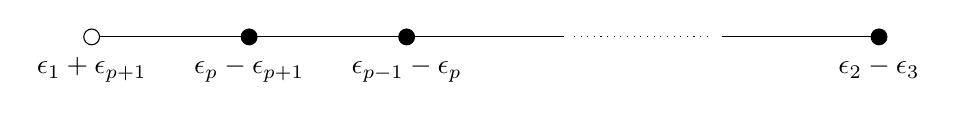
\begin{tikzpicture}
\draw (0 cm,0) -- (6 cm,0);
\draw (8 cm,0) -- (10 cm,0);
\draw[fill=white] (0 cm, 0 cm) circle (.1cm) node[below=4pt]{$\epsilon_{1} + \epsilon_{p+1}$};
\draw[fill=black] (2 cm, 0 cm) circle (.1cm) node[below=4pt]{$\epsilon_{p} - \epsilon_{p+1}$};
\draw[fill=black] (4 cm, 0 cm) circle (.1cm) node[below=4pt]{$\epsilon_{p-1} - \epsilon_{p}$};
\node (node_a) at (6 cm, 0 cm) {};
\node (node_b) at (8 cm, 0 cm) {};
\draw[fill=black] (10 cm, 0 cm) circle (.1cm) node[below=4pt]{$\epsilon_{2} - \epsilon_{3}$};
\draw [dotted] (node_a) to (node_b);
\end{tikzpicture}  
  \caption{The reduced hermitian symmetric pair $(\mathfrak{g}_\lambda, \mathfrak{k}_\lambda)$}
\end{figure}
  
The integral cone is in this case
  \[
    C = \{ a_1\omega_1 + a_{p+1}\omega_{p+1} + \cdots + a_n \omega_n \,|\, a_1 + 2( a_{p+1} + \cdots + a_{n-1}) + a_n = 0 \}
  \]
  and one can easily check that $\Psi^+_\lambda = \Psi^+_{\lambda+\mu}$ for all $\mu \in C$ and thus the translation theorem \ref{thm:translation} applies.
  
\begin{figure}[H]
  \centering
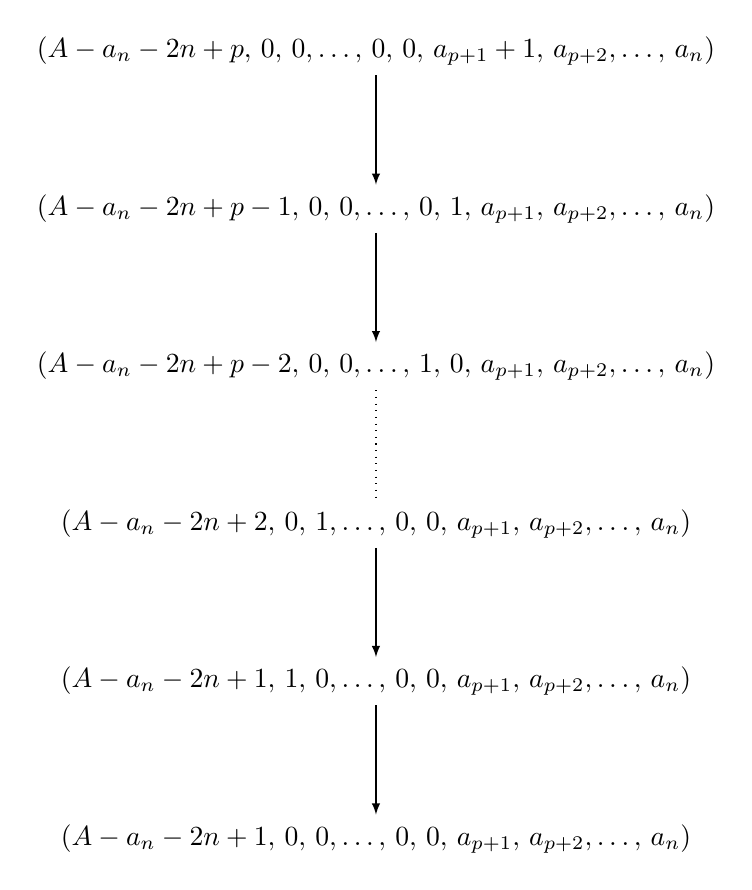
\begin{tikzpicture}[>=latex,line join=bevel,]
%%
  \node (node_0) at (0,10) [draw,draw=none] {$\left(A  - a_{n} - 2n + p,\,0,\,0,\ldots,\,0,\,0,\,a_{p+1}+1,\,a_{p+2},\ldots,\,a_{n}\right)$};
  \node (node_1) at (0,8) [draw,draw=none] {$\left(A  - a_{n} - 2n + p-1,\,0,\,0,\ldots,\,0,\,1,\,a_{p+1},\,a_{p+2},\ldots,\,a_{n}\right)$};
  \node (node_2) at (0,6) [draw,draw=none] {$\left(A  - a_{n} - 2n + p-2,\,0,\,0,\ldots,\,1,\,0,\,a_{p+1},\,a_{p+2},\ldots,\,a_{n}\right)$};
  \node (node_3) at (0,4) [draw,draw=none] {$\left(A - a_{n} - 2n+2,\,0,\,1,\ldots,\,0,\,0,\,a_{p+1},\,a_{p+2},\ldots,\,a_{n}\right)$};
  \node (node_4) at (0,2) [draw,draw=none] {$\left(A  - a_{n} - 2n + 1,\,1,\,0,\ldots,\,0,\,0,\,a_{p+1},\,a_{p+2},\ldots,\,a_{n}\right)$};  
  \node (node_5) at (0,0) [draw,draw=none] {$\left(A  - a_{n} - 2n + 1,\,0,\,0,\ldots,\,0,\,0,\,a_{p+1},\,a_{p+2},\ldots,\,a_{n}\right)$};

  \draw [black,->] (node_0) edge (node_1);
  \draw [black,->] (node_1) edge (node_2);
  \draw [dotted] (node_2) to (node_3);
  \draw [black,->] (node_3) edge (node_4);
  \draw [black,->] (node_4) edge (node_5);
%
\end{tikzpicture}
  \caption{Nilpotent cohomology / BGG resolution, $A = -2(a_{p+1} + \cdots + a_{n-1})$}
\end{figure}
      
 \item $\lambda = -(n+1)\omega_1 + 2\omega_n $\\
    Scalar products of positive noncompact roots with $\lambda+\rho$
      \begin{align*}
	(\epsilon_1, \lambda+\rho) &= -\frac{1}{2} \\
	(\epsilon_1+\epsilon_j,\lambda+\rho) &=  n+1-j \\
	(\epsilon_1-\epsilon_j,\lambda+\rho) &= -n-2+j
      \end{align*}
    show that the set of singular roots is again empty $\Psi^+_\lambda = \emptyset$ and the set of generating roots is $\roots^+_{n,\lambda} = \{\epsilon_1 + \epsilon_j \,|\, 1<j\leq n \}$. The generated root subsystem of type $A_{n-1}$ is
    \[
      \roots_\lambda = \{ \pm(\epsilon_1 + \epsilon_j \,|\, 1<j\leq p+1 \} \cup \{ \epsilon_i - \epsilon_j \,|\, 1 < i,j \leq p+1 \et i\neq j \}.
    \]

The integral cone is in this case \[C = \{t(-\omega_1 + \omega_n) \,|\, t\in\mathbb{N}_0 \}\] and $\Psi^+_\lambda = \Psi^+_{\lambda+\mu}$ for all $\mu \in C$.      


\begin{figure}[H]
  \centering
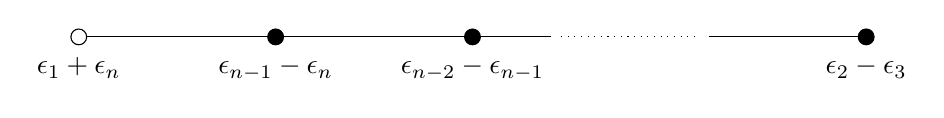
\begin{tikzpicture}
\draw (0 cm,0) -- (6 cm,0);
\draw (8 cm,0) -- (10 cm,0);
\draw[fill=white] (0 cm, 0 cm) circle (.1cm) node[below=4pt]{$\epsilon_{1} + \epsilon_{n}$};
\draw[fill=black] (2.5 cm, 0 cm) circle (.1cm) node[below=4pt]{$\epsilon_{n-1} - \epsilon_{n}$};
\draw[fill=black] (5 cm, 0 cm) circle (.1cm) node[below=4pt]{$\epsilon_{n-2} - \epsilon_{n-1}$};
\node (node_a) at (6 cm, 0 cm) {};
\node (node_b) at (8 cm, 0 cm) {};
\draw[fill=black] (10 cm, 0 cm) circle (.1cm) node[below=4pt]{$\epsilon_{2} - \epsilon_{3}$};
\draw [dotted] (node_a) to (node_b);
\end{tikzpicture}  
  \caption{The reduced hermitian symmetric pair $(\mathfrak{g}_\lambda, \mathfrak{k}_\lambda)$}
\end{figure}  

\begin{figure}[H]
  \centering
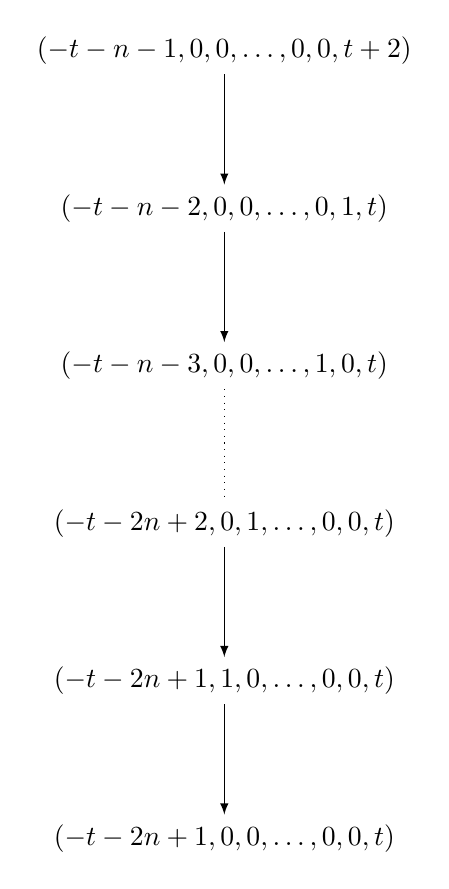
\begin{tikzpicture}[>=latex,line join=bevel,]
%%
  \node (node_0) at (0,10) [draw,draw=none] {$\left(-t-n-1, 0, 0, \ldots, 0, 0, t+2\right)$};
  \node (node_1) at (0,8) [draw,draw=none] {$\left(-t-n-2, 0, 0, \ldots, 0, 1, t \right)$};
  \node (node_2) at (0,6) [draw,draw=none] {$\left(-t-n-3, 0, 0, \ldots, 1, 0, t \right)$};
  \node (node_3) at (0,4) [draw,draw=none] {$\left(-t-2n+2, 0, 1, \ldots, 0, 0, t \right)$};
  \node (node_4) at (0,2) [draw,draw=none] {$\left(-t-2n+1, 1, 0, \ldots, 0, 0, t \right)$};
  \node (node_5) at (0,0) [draw,draw=none] {$\left(-t-2n+1, 0, 0, \ldots, 0, 0, t \right)$};

  \draw [black,->] (node_0) edge (node_1);
  \draw [black,->] (node_1) edge (node_2);
  \draw [dotted] (node_2) to (node_3);
  \draw [black,->] (node_3) edge (node_4);
  \draw [black,->] (node_4) edge (node_5);
%
\end{tikzpicture}
  \caption{Nilpotent cohomology / BGG resolution}
\end{figure}

 \item $\lambda = 0 $\\
       In this case the scalar products of positive roots with $\lambda+\rho$ are of course given by \eqref{eq:Bn_rho_scalar_posroots} and there are no singular roots $\Psi^+_\lambda = \emptyset$. We have $\roots^+_{n,\lambda} = \roots^+_n$, the root subsystem is
       \[
        \roots_\lambda = \roots
       \]
       and the Kostant's formula applies.
       
 \item $\lambda = (\frac{3}{2} - n)\omega_1  $\\
      The scalar products of positive noncompact roots with $\lambda+\rho$ are
      \begin{align*}
	(\epsilon_1, \lambda+\rho) &= 1 \\
	(\epsilon_1+\epsilon_j,\lambda+\rho) &=  n+\frac{3}{2}-j \\
	(\epsilon_1-\epsilon_j,\lambda+\rho) &= -n + \frac{1}{2} + j.
      \end{align*}
      The set of singular roots is empty $\Psi^+_\lambda = \emptyset$ and the integrality conditions of the definition \ref{def:cohomology_roots} imply that $\roots^+_{n,\lambda} = \{ \epsilon_1 \}$. It follows that
      \[
       \roots_\lambda = \{ \pm \epsilon_1 \} 
      \]
      and that all the nontrivial cohomologies are contained in the table \ref{tbl:so_odd}.
      
 \item $\lambda = -(n-\frac{1}{2})\omega_1 + \omega_n  $\\
      Sscalar products of positive noncompact roots with $\lambda+\rho$
      \begin{align*}
	(\epsilon_1, \lambda+\rho) &= \frac{1}{2} \\
	(\epsilon_1+\epsilon_j,\lambda+\rho) &=  n+\frac{3}{2}-j \\
	(\epsilon_1-\epsilon_j,\lambda+\rho) &= -n-\frac{1}{2}+j
      \end{align*}
      again show that there are no singular roots $\Psi^+_\lambda = \emptyset$ and since $\epsilon_1^\vee = 2\epsilon_1$ we have $\roots^+_{n,\lambda} = \{ \epsilon_1 \}$. This yields the subsystem
      \[
       \roots_\lambda = \{ \pm \epsilon_1 \} 
      \]
      which is of type $A_1$ and the nontrivial cohomologies are given by table \ref{tbl:so_odd}. 
\end{enumerate}

%%%%%%%%%%%% ALL ROOTS
% 
% Before we compute the cohomology we first do some preliminary calculations and write down the scalar products of positive roots $\roots^+ = \{ \epsilon_i \pm \epsilon_j \,|\, 1\leq i < j \leq n \} \cup \{ \epsilon_i \,|\, 1\leq i \leq n\}$ with $\rho$
% \begin{equation}\label{eq:Bn_rho_scalar_posroots}
%  \begin{split}
%   (\epsilon_i, \rho) & = n + \frac{1}{2} - i \\
%   (\epsilon_i + \epsilon_j, \rho) & = n + \frac{1}{2} - i + n + \frac{1}{2} - j = 2n+1-i-j \\
%   (\epsilon_i - \epsilon_j, \rho) & = n + \frac{1}{2} - i - (n + \frac{1}{2} - j) = j - i.
%  \end{split}
% \end{equation}
% 
% \begin{enumerate}
%  \item $\lambda = (p-2n) \omega_1 + \omega_{p+1}$\\
%       The scalar products of positive roots with $\lambda+\rho$
%       \begin{gather*}
% 	(\epsilon_i, \lambda+\rho) = \begin{cases}
% 	                              p-n+\frac{1}{2}, & i=1\\
% 	                              \frac{3}{2} + n -i, & 1 < i \leq p+1 \\
% 	                              \frac{1}{2} + n - i, & p+1 < i 
% 	                             \end{cases}\\
% 	(\epsilon_i+\epsilon_j,\lambda+\rho) = \begin{cases} 
% 	                                        p+2-j, & i=1, 1<j\leq p+1\\
% 						2n+3-i-j,& 1<i<j\leq p+1 \\
% 						2n+2 -i -j, & 1<i\leq p+1 <j \leq n \\
% 						2n+1-i-j, & p+1 < i < j \leq n
% 	                                       \end{cases}\\
% 	(\epsilon_i-\epsilon_j,\lambda+\rho) = \begin{cases}
% 	                                        p+2n+j-i, & i=1, 1<j\leq p+1\\
% 						j-i,& 1<i<j\leq p+1 \\
% 						1+j-i, & 1<i\leq p+1 <j \leq n \\
% 						j-i, & p+1 < i < j \leq n.
% 	                                       \end{cases}\\
%       \end{gather*}
%  \item $\lambda = -(n+1)\omega_1 + 2\omega_n $\\
%        The scalar products of positive roots with $\lambda+\rho$
%       \begin{gather*}
% 	(\epsilon_i, \lambda+\rho) = \begin{cases}
% 	                              -\frac{1}{2}, & i = 1 \\
% 	                              n+\frac{3}{2} - i, & 1<i\leq n
% 	                             \end{cases}\\
% 	(\epsilon_i+\epsilon_j,\lambda+\rho) = \begin{cases}
% 	                                        n+1-j, & i=1, 1<j\leq n\\
% 	                                        2n+3-i-j, & 1 < i < j \leq n
% 	                                       \end{cases}\\
% 	(\epsilon_i-\epsilon_j,\lambda+\rho) = \begin{cases}
% 	                                        -n-2+j, & i=1, 1<j\leq n \\
% 	                                        j-i, & 1 < i < j \leq n
% 	                                       \end{cases}
%       \end{gather*}
%  \item $\lambda = 0 $\\
%        In this case the scalar products of positive roots with $\lambda+\rho$ are of course given by \eqref{eq:Bn_rho_scalar_posroots}.
%  \item $\lambda = (\frac{3}{2} - n)\omega_1  $\\
%        The scalar products of positive roots with $\lambda+\rho$
%       \begin{gather*}
% 	(\epsilon_i, \lambda+\rho) = \\
% 	(\epsilon_i+\epsilon_j,\lambda+\rho) = \\
% 	(\epsilon_i-\epsilon_j,\lambda+\rho) =
%       \end{gather*}
%  \item $\lambda = -(n-\frac{1}{2})\omega_1 + \omega_n  $\\
%        The scalar products of positive roots with $\lambda+\rho$
%       \begin{gather*}
% 	(\epsilon_i, \lambda+\rho) = \\
% 	(\epsilon_i+\epsilon_j,\lambda+\rho) = \\
% 	(\epsilon_i-\epsilon_j,\lambda+\rho) =
%       \end{gather*}
% \end{enumerate}


\begin{figure}[H]
  \centering
  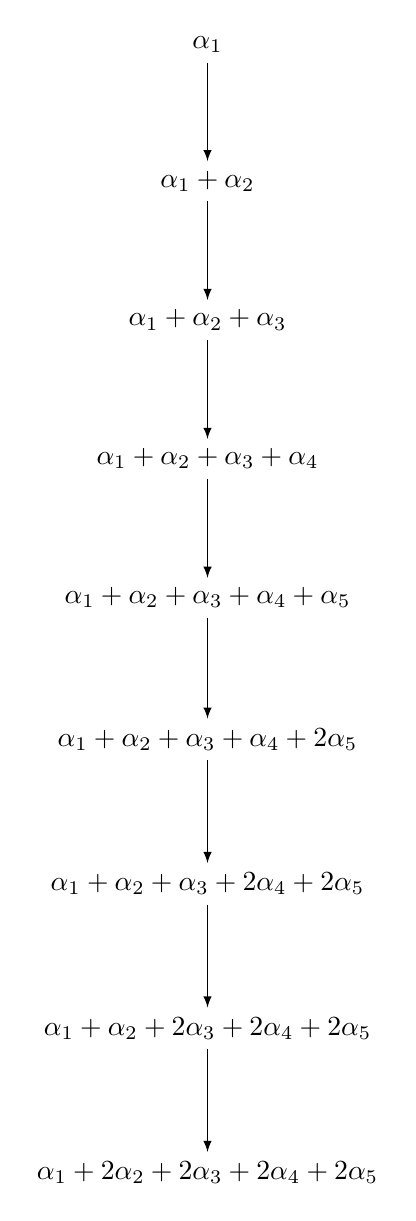
\begin{tikzpicture}[>=latex,line join=bevel,]
%%
\node (alpha1) at (64bp,414bp) [draw,draw=none] {$\alpha_{1}$};
  \node (alpha1+alpha2+alpha3+alpha4+2*alpha5) at (64bp,164bp) [draw,draw=none] {$\alpha_{1} + \alpha_{2} + \alpha_{3} + \alpha_{4} + 2\alpha_{5}$};
  \node (alpha1+alpha2) at (64bp,365bp) [draw,draw=none] {$\alpha_{1} + \alpha_{2}$};
  \node (alpha1+alpha2+alpha3+alpha4) at (64bp,265bp) [draw,draw=none] {$\alpha_{1} + \alpha_{2} + \alpha_{3} + \alpha_{4}$};
  \node (alpha1+alpha2+alpha3+2*alpha4+2*alpha5) at (64bp,112bp) [draw,draw=none] {$\alpha_{1} + \alpha_{2} + \alpha_{3} + 2\alpha_{4} + 2\alpha_{5}$};
  \node (alpha1+alpha2+alpha3) at (64bp,315bp) [draw,draw=none] {$\alpha_{1} + \alpha_{2} + \alpha_{3}$};
  \node (alpha1+alpha2+alpha3+alpha4+alpha5) at (64bp,215bp) [draw,draw=none] {$\alpha_{1} + \alpha_{2} + \alpha_{3} + \alpha_{4} + \alpha_{5}$};
  \node (alpha1+alpha2+2*alpha3+2*alpha4+2*alpha5) at (64bp,60bp) [draw,draw=none] {$\alpha_{1} + \alpha_{2} + 2\alpha_{3} + 2\alpha_{4} + 2\alpha_{5}$};
  \node (alpha1+2*alpha2+2*alpha3+2*alpha4+2*alpha5) at (64bp,8bp) [draw,draw=none] {$\alpha_{1} + 2\alpha_{2} + 2\alpha_{3} + 2\alpha_{4} + 2\alpha_{5}$};
  \draw [black,->] (alpha1) ..controls (64bp,401.84bp) and (64bp,391.19bp)  .. (alpha1+alpha2);
  \draw [black,->] (alpha1+alpha2+alpha3+alpha4+alpha5) ..controls (64bp,201.52bp) and (64bp,190.94bp)  .. (alpha1+alpha2+alpha3+alpha4+2*alpha5);
  \draw [black,->] (alpha1+alpha2+alpha3+2*alpha4+2*alpha5) ..controls (64bp,97.763bp) and (64bp,87.065bp)  .. (alpha1+alpha2+2*alpha3+2*alpha4+2*alpha5);
  \draw [black,->] (alpha1+alpha2+2*alpha3+2*alpha4+2*alpha5) ..controls (64bp,45.763bp) and (64bp,35.065bp)  .. (alpha1+2*alpha2+2*alpha3+2*alpha4+2*alpha5);
  \draw [black,->] (alpha1+alpha2+alpha3+alpha4+2*alpha5) ..controls (64bp,149.76bp) and (64bp,139.06bp)  .. (alpha1+alpha2+alpha3+2*alpha4+2*alpha5);
  \draw [black,->] (alpha1+alpha2+alpha3) ..controls (64bp,301.29bp) and (64bp,291.02bp)  .. (alpha1+alpha2+alpha3+alpha4);
  \draw [black,->] (alpha1+alpha2) ..controls (64bp,351.29bp) and (64bp,341.02bp)  .. (alpha1+alpha2+alpha3);
  \draw [black,->] (alpha1+alpha2+alpha3+alpha4) ..controls (64bp,251.29bp) and (64bp,241.02bp)  .. (alpha1+alpha2+alpha3+alpha4+alpha5);
%
\end{tikzpicture} 
	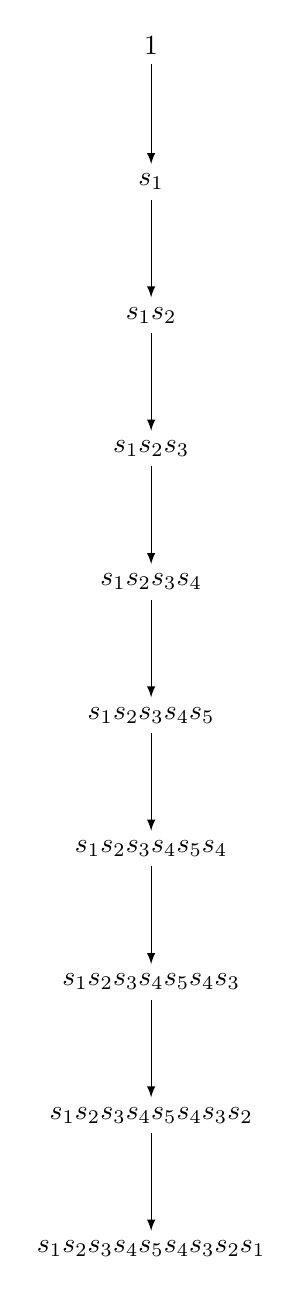
\begin{tikzpicture}[>=latex,line join=bevel,]
%%
  \node (s1) at (44bp,390bp) [draw,draw=none] {$s_{1}$};
  \node (s1*s2*s3*s4*s5*s4*s3) at (44bp,102bp) [draw,draw=none] {$s_{1}s_{2}s_{3}s_{4}s_{5}s_{4}s_{3}$};
  \node (s1*s2*s3*s4*s5*s4*s3*s2*s1) at (44bp,6bp) [draw,draw=none] {$s_{1}s_{2}s_{3}s_{4}s_{5}s_{4}s_{3}s_{2}s_{1}$};
  \node (1) at (44bp,439bp) [draw,draw=none] {$1$};
  \node (s1*s2*s3*s4*s5*s4*s3*s2) at (44bp,54bp) [draw,draw=none] {$s_{1}s_{2}s_{3}s_{4}s_{5}s_{4}s_{3}s_{2}$};
  \node (s1*s2*s3*s4*s5*s4) at (44bp,150bp) [draw,draw=none] {$s_{1}s_{2}s_{3}s_{4}s_{5}s_{4}$};
  \node (s1*s2*s3) at (44bp,294bp) [draw,draw=none] {$s_{1}s_{2}s_{3}$};
  \node (s1*s2) at (44bp,342bp) [draw,draw=none] {$s_{1}s_{2}$};
  \node (s1*s2*s3*s4*s5) at (44bp,198bp) [draw,draw=none] {$s_{1}s_{2}s_{3}s_{4}s_{5}$};
  \node (s1*s2*s3*s4) at (44bp,246bp) [draw,draw=none] {$s_{1}s_{2}s_{3}s_{4}$};
  \draw [black,->] (s1*s2*s3*s4*s5*s4*s3*s2) ..controls (44bp,41.554bp) and (44bp,31.067bp)  .. (s1*s2*s3*s4*s5*s4*s3*s2*s1);
  \draw [black,->] (s1*s2*s3*s4*s5) ..controls (44bp,185.55bp) and (44bp,175.07bp)  .. (s1*s2*s3*s4*s5*s4);
  \draw [black,->] (1) ..controls (44bp,425.83bp) and (44bp,415.21bp)  .. (s1);
  \draw [black,->] (s1*s2*s3*s4*s5*s4) ..controls (44bp,137.55bp) and (44bp,127.07bp)  .. (s1*s2*s3*s4*s5*s4*s3);
  \draw [black,->] (s1*s2*s3) ..controls (44bp,281.55bp) and (44bp,271.07bp)  .. (s1*s2*s3*s4);
  \draw [black,->] (s1) ..controls (44bp,377.55bp) and (44bp,367.07bp)  .. (s1*s2);
  \draw [black,->] (s1*s2) ..controls (44bp,329.55bp) and (44bp,319.07bp)  .. (s1*s2*s3);
  \draw [black,->] (s1*s2*s3*s4) ..controls (44bp,233.55bp) and (44bp,223.07bp)  .. (s1*s2*s3*s4*s5);
  \draw [black,->] (s1*s2*s3*s4*s5*s4*s3) ..controls (44bp,89.554bp) and (44bp,79.067bp)  .. (s1*s2*s3*s4*s5*s4*s3*s2);
%
\end{tikzpicture} 
  \caption{Poset of noncompact roots for $\mathrm{SO}(2,9)$}
\end{figure} 


